\documentclass[12pt]{article}

\usepackage[brazil]{babel}
\usepackage[utf8]{inputenc}

\usepackage{color}
\usepackage{multirow}
\usepackage{amssymb}
\usepackage{subfigure}
\usepackage{graphicx}
\usepackage{caption2}
\usepackage{setspace}
\usepackage{amsmath}
\usepackage{url}
\usepackage{makeidx}
\usepackage{subfigure}
\usepackage{epsfig}
\usepackage{changebar}
\usepackage{graphicx}
\usepackage{caption2}
\usepackage{setspace}
\usepackage{indentfirst}
\usepackage{array}
\usepackage{delarray}
\usepackage{calc}
\usepackage{fancyhdr}
\usepackage{textcomp}
\usepackage{theorem}
\usepackage{amssymb}
\usepackage[margin=0.7in]{geometry}

\oddsidemargin -.25in \evensidemargin -.25in \topmargin .05in
\textheight 52pc 
\textwidth 40pc   %6.8
\headheight 0.2in \headsep 0.2in 
\parindent 0.2in

\begin{document}

\title{Estrutura de Dados 2}
\date{\today}

\maketitle

\vspace{40pt}

\begin{center}
Relatório Trabalho Prático
\end{center}

\vspace{80pt}

%==================================
\section{Identificação do relatório}
%==================================

\vspace{20pt} \noindent

\vspace{20pt} 

\textbf{Equipe}: Kelvin James de Souza Martins - RA: 1986813\\
        \hspace*{65pt}{Rafael Lammel Marinheiro - RA: 1986856}

\vspace{20pt} 

\textbf{Curso}: Sistemas de Informação

\vspace{20pt}

\textbf{Departamento}: DAINF

\vspace{20pt} 

\textbf{Instituição}: Universidade Tecnológica Federal do Paraná (UTFPR).
\newpage
%=================
\section{Introdução}
%=================

Neste projeto a dupla implementou operações de remoção e inserção em uma árvore B, tal como um arquivo Makefile. A árvore B se define como uma árvore que não precisa acessar o disco diversas vezes, pois cada nó possui um vetor de tamanho máximo $2*T-1$ e mínimo $T-1$ sendo T um grau mínimo definido pelo programador. As regras de inserção são baseadas nas regras da árvore binária de busca (ABB), onde uma nova chave deve ser colocada no filho esquerdo sendo menor ou caso contrário no filho direito (isso é um processo recursivo). A árvore B também se destaca na sua complexidade, sendo $log N$, se formos fazer uma comparação com a árvore AVL, uma análise precipitada, poderia ter uma conclusão de que elas não possuem diferença em desempenho, mas a árvore B consegue armazenar um maior número de dados com altura menor, então o N da complexidade também é menor.
\par Nas proximas seções descreveremos o processo de desenvolvimento com algumas ilustrações das etapas.
\section{Instruções}
O código é acompanhado de um arquivo Makefile para sua execução. Ele imprime duas árvore B, uma com chaves "int" e grau mínimo 3 e outra com chaves "char" e grau mínimo 2. Ela está configurada para rodar com "char".
\par Para trocar o tipo e o grau mínimo da árvore, é necessário modificar os arquivos arvoreb.h, mainArvoreb.c, printArvoreb.c e removeArvoreb.c. No arquivo arvoreb.h, altere onde estão circulados em vermelho na imagem para o tipo e grau mínimo desejado.

\begin{figure}[!h]
\centering
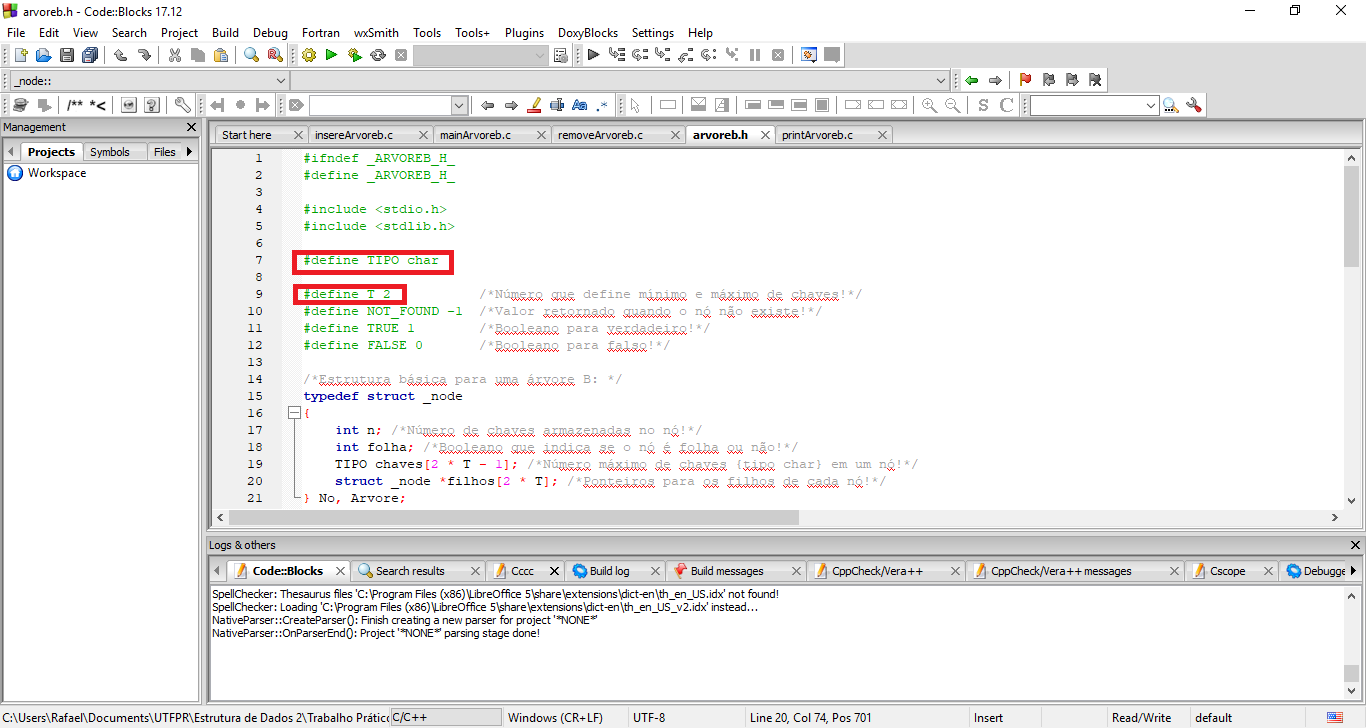
\includegraphics[width=6in]{relatorio/imagens/imgMudarTipoH.png}
\end{figure}

\newpage

\par No arquivo mainArvoreb.c, dentro da main, remova os comentários da função equivalente ao tipo que você quer (Numérico = "int", Alfabeto = "char"), como indica a figura abaixo no retângulo vermelho:

\begin{figure}[!h]
\centering
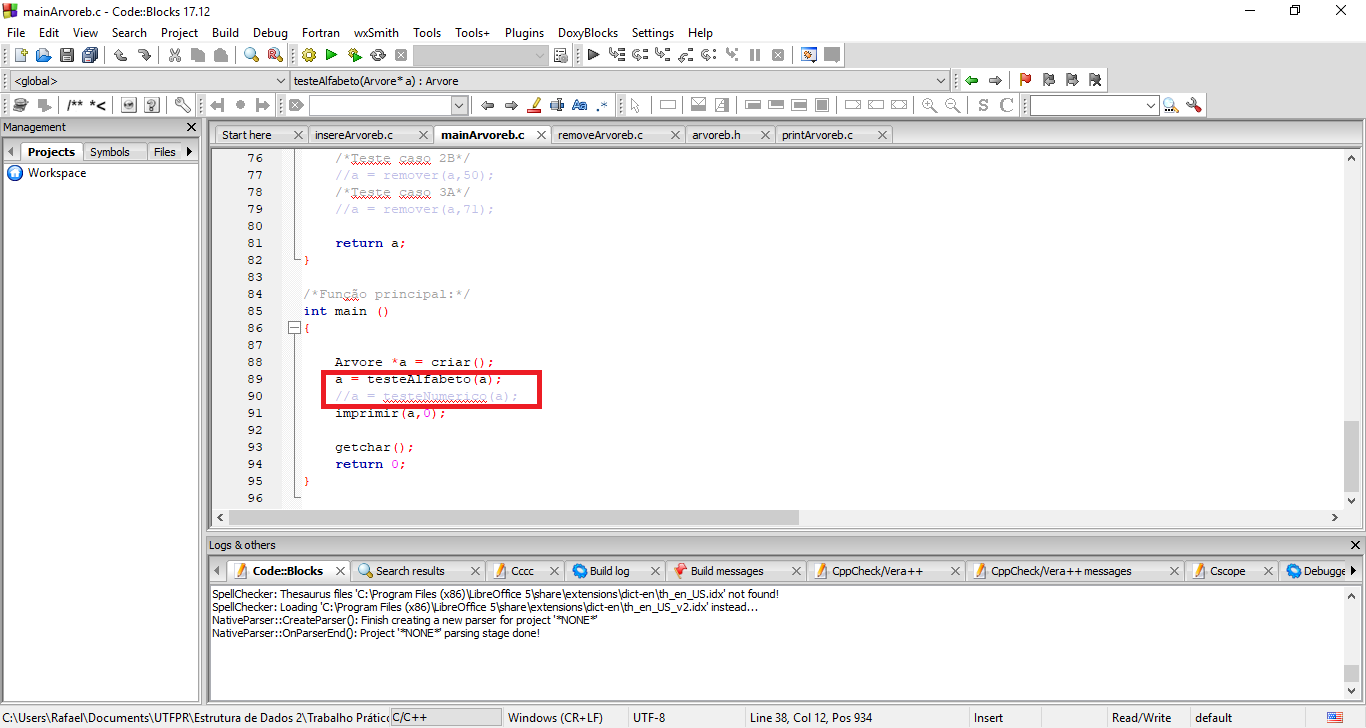
\includegraphics[width=6in]{relatorio/imagens/imgMudarTipoMain.png}
\end{figure}

\par Em printArvoreb.c, basta alterar alterar o tipo de sáida do printf circulado em vermelho na imagem abaixo para corresponder ao tipo da sua árvore:

\begin{figure}[!h]
\centering
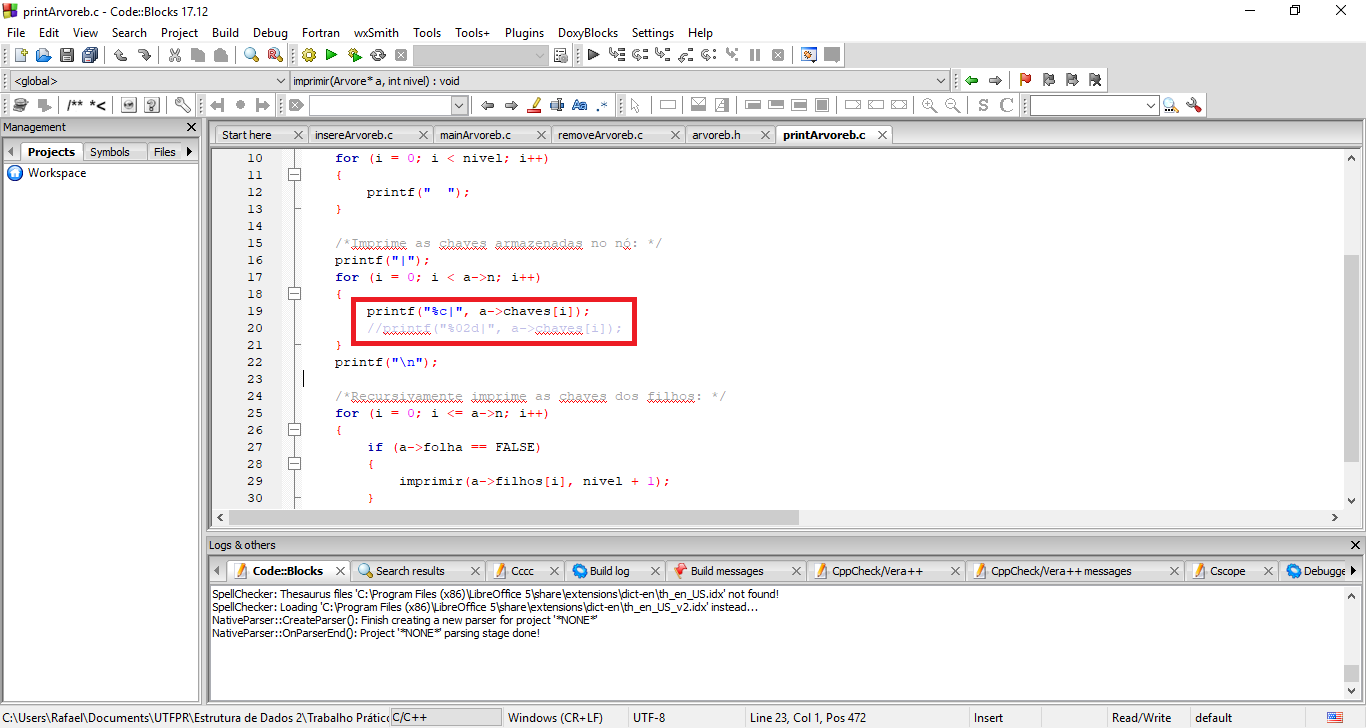
\includegraphics[width=6in]{relatorio/imagens/imgMudarTipoPrint.png}
\end{figure}
\newpage
\par Enfim, para removeArvoreb.c, basta fazer a mesma coisa que em printArvoreb.c:

\begin{figure}[!h]
\centering
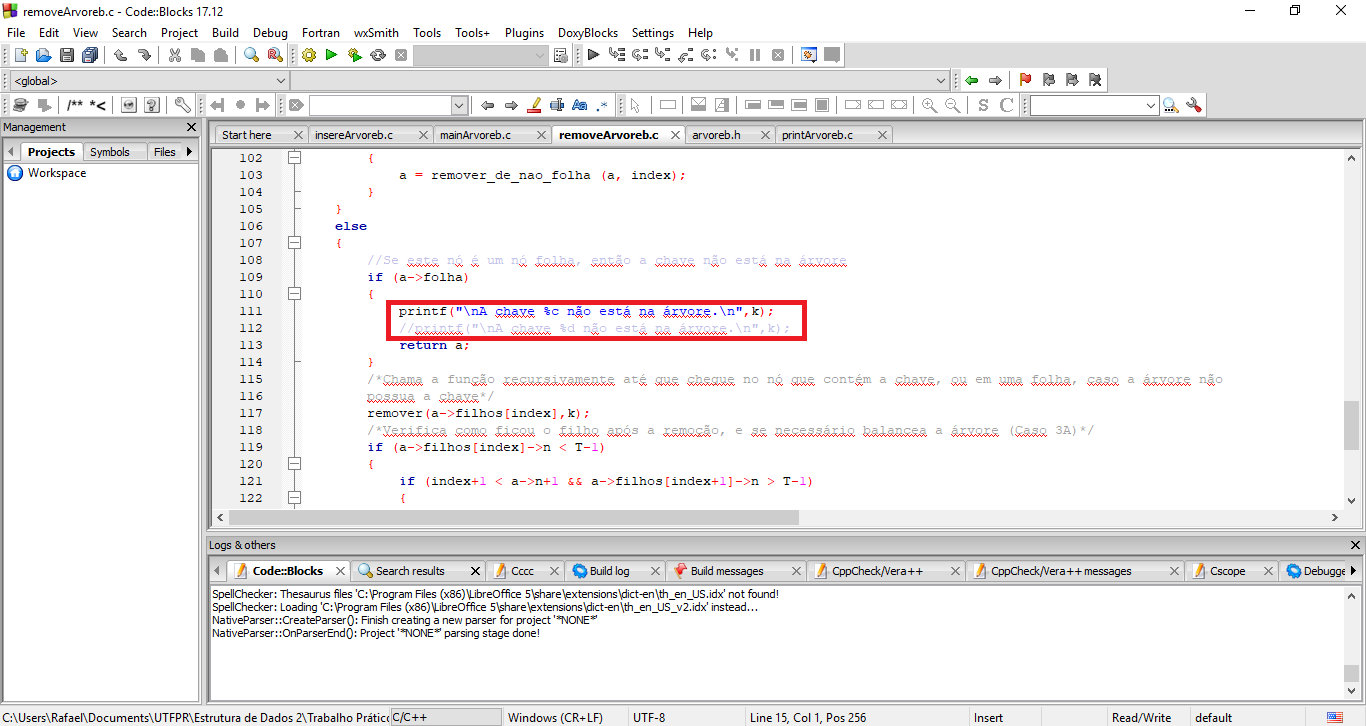
\includegraphics[width=6in]{relatorio/imagens/imgMudarTipoRemove.png}
\end{figure}
\par Nosso código também vem com alguns testes de remoção. Eles se encontram dentro das funções testeAlfabeto e testeNumerico, ambas com seus respectivos testes. Para realizar uma remoção, basta tirar do comentário qualquer uma das chamadas de remoção, mas como nosso programa só implementou 4 formas de remoção, pode causar problemas rodar mais do que uma na mesma execução. Recomendamos que se teste uma por vez.

\begin{figure}[!h]
\centering
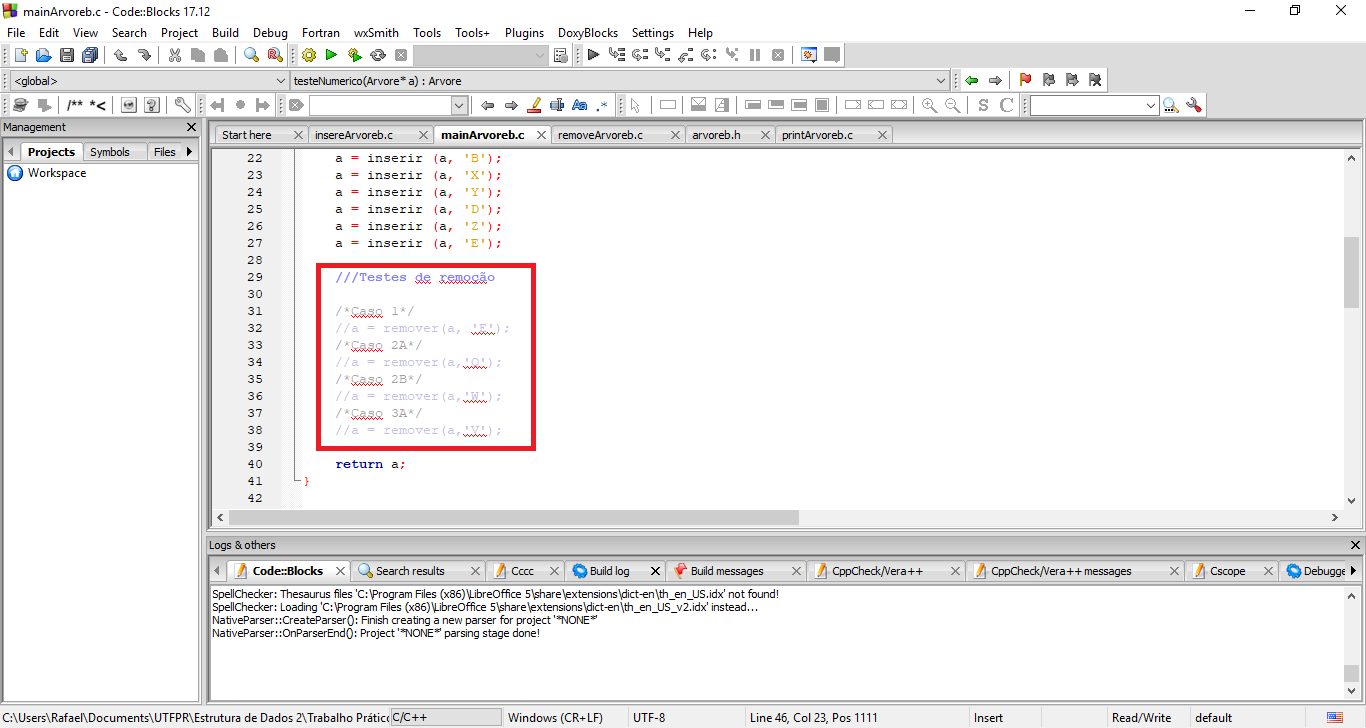
\includegraphics[width=6in]{relatorio/imagens/imgTestesRemocaoChar.png}
\end{figure}

\begin{figure}[!h]
\centering
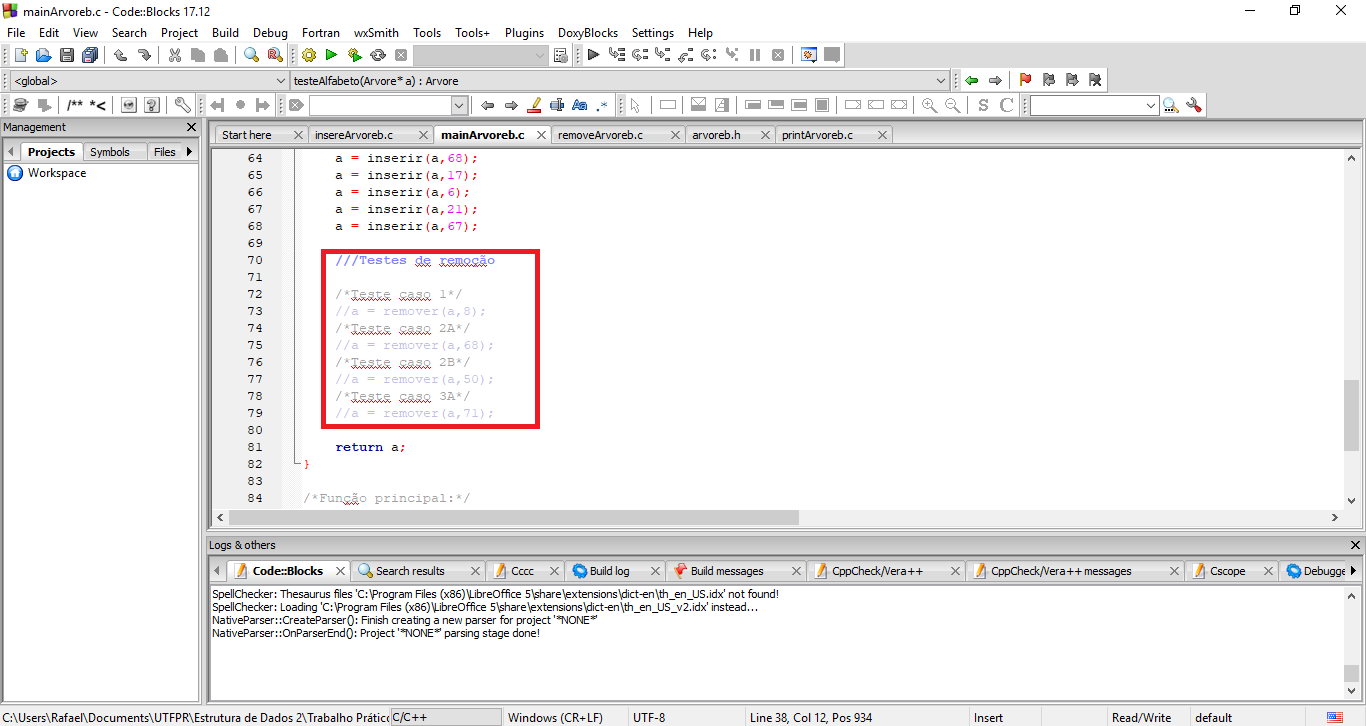
\includegraphics[width=6in]{relatorio/imagens/imgTestesRemocaoInt.png}
\end{figure}
\newpage
\section{Makefile}
A construção do nosso Makefile foi rápida e teve poucos problemas. conseguimos entender rápidamente a estrutura simples.
\begin{verbatim}
[Arquivo a ser gerado] : [Dependências - Arquivos que servem como fonte]
    [O código que deve ser executado pelo terminal]
\end{verbatim}
Tivemos alguns problemas com o TAB, que precisa necessariamente ter 4 espaços. Nós usamos o editor Atom que tem o TAB configurado como 2 espaços. Alteramos isso, e nosso Makefile funcionou perfeitamente.
\par Posteriormente tivemos problemas, que a priori achamos que fosse no código, mas logo percebemos que era no Makefile: toda vez que alteravamos o código para testes de chars para ints ou vice versa, o programa não executava da forma esperada. Depois de quase dois dias revisando, percebemos que nosso .h não é compilado, mas ele é usado em todos os nossos .c. Quando mudamos o tipo da váriavel alteramos o .h, mas apenas alguns .c, fazendo com que alguns .c fiquem com o .h antigo e outros com o novo. Resolvemos isso simplesmente adicionando o .h como dependência de todos os .o, como visto no exemplo abaixo:

\begin{figure}[!h]
\centering
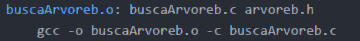
\includegraphics[width=5in]{relatorio/imagens/imgMakefile.png}
\end{figure}

\par Isso foi tudo que fizemos com o Makefile. Na próxima seção discutiremos sobre a inserção.
%===============================
\section{Inserção}
%===============================
A dupla começou o desenvolvimento da árvore pela inserção de elementos, pois já tinhamos a base no livro indicado pela professora. A implementação foi básicamente transformar aquele pseudo-código no nosso código C. Tivemos alguns problemas em relação ao tamanho dos vetores, já que no pseudo-código eles começavam pelo número 1 e na linguagem C começa-se pelo 0.
\par Nas primeiras versões do nosso código, alguns problemas foram apresentados ao dividir um nó, não verificavamos se o lugar apropriado para o novo elemento era o nó esquerdo ou direito, por consequência disso, todo novo elemento automaticamente ia para o nó esquerdo, demoramos para localizar o erro, porém após identificado, a solução foi elementar.  

\begin{figure}[!h]
\centering
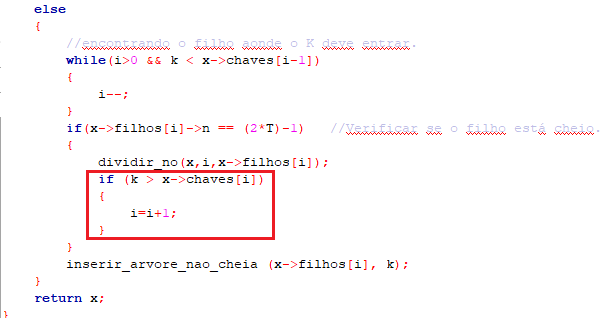
\includegraphics[width=6in]{relatorio/imagens/imgIfInsercao.png}
\end{figure}
\section{Remoção}
A remoção foi a parte mais complicada desse projeto. Como era necessário escolher 4 das 6 formas de remoção apresentadas, a dupla analisou as formas mais simples para realizar primeiro.

\subsection{Caso 1}
Começamos pelo caso 1, que é quando queremos remover a chave de uma folha que tem pelo menos T chaves. Essa parte foi super simples e a implementação foi feita em poucos minutos. Basicamente chegamos no nó que contém a chave, removemos e rearranjamos o nó se necessário.

\subsection{Caso 2A e 2B}
Quando removemos algo de um nó não folha, verificamos se algum dos dois filhos tem pelo menos T chaves, se o da esquerda tiver, é feito o caso 2A, onde pegamos o filho máximo(maior elemento da sub-árvore) da esquerda e trocamos com o elemento que será removido, após essa troca, passamos a tratar a remoção no elemento máximo(por conta das propriedades da árvore B, ele sempre estará em um nó folha), no caso 2B, o filho a direita é quem possui pelo menos T chaves, então ao invés de pegarmos o máximo, fazemos a troca com o mínimo e passamos a tratar a remoção nele, assim como no caso 2A. 
\par
Percebe-se que os casos são extremamente parecidos, por esse motivo decidimos que seria melhor deixar ambas na mesma seção para facilitar na descrição.
\subsection{Caso 3A}
Esse caso acontece quando a remoção é feita em um nó folha que possui o mínimo de chaves($T-1$) e se pelo menos um dos irmãos possuem pelo menos T chaves, ao remover o elemento, o pai desce para balancear o nó, no irmão pegamos o elemento máximo ou mínimo(depende de qual irmão, esquerdo ou direito) e colocamos no lugar aonde anteriormente o pai estava.
\par
Na hora da implementação, nos atentamos á um caso específico, o elemento que estará sendo removido, pode estar em alguma das extremidades da subárvore, nesse caso, dependendo de qual lado está, verificamos a quantidade de elementos de somente um irmão. 


\end{document}